\chapter{Experiment Design}

    we have conducted two experiments in this paper. First we are curious about whether the economics variables can predict the intra-day data of currency market, also gives a very beginning look of innovations methods applying on our problem.
    Second we apply our model on Forex carry strategy, which only put a lot of attention on the tomorrow's currency moment, and inherent the experience from our previous experiment to improve our model.


\section{Data Description}

For our first experiment we use one-month historical currency data in million-second based, and Wharton Research Data Services Fama-French, Coild-oil in daily based.

%https://pepperstone.com/mt4-forex-trading/mt4-tick-chart-history-data.php
%http://research.stlouisfed.org/fred2/series/DCOILWTICO
\begin{enumerate}
\item{GBP/JPY: tick-by-tick data in million-seconds for 2014-11}
\item{Crude Oil Prices: West Texas Intermediate (WTI) in daily frequency obtain from 1986-2014}
\item{Fama French \& Liquidity Factors: in daily frequency
from 2005-01-01 to 2015-03-31}
\item{The CBOE (Chicago Board Options Exchange) Volatility Index in daily frenquency}
\item{Current exchange rate Gold (XAU) to US DOLLAR (USD): tick-by-tick data in million-sec frequency for 2014-11}
\end{enumerate}
\newpage

    Since there are no representative papers support which economic factors are promising for forecasting exchange rate movement, or Forex carry daily return movement. We carry out an exploratory experiment to give a very look into our problem, which economic factors could give us a glance of future.
    
% Explain our data sets
    
    The only promising forecasting factor is currency forward. Financial theory suggests that under no arbitrage condition, the relation between forward rate and future exchange rate can be written as follow.

    For more deeply concern is that we apply the same concept from the paper[], using risk metric as independent variables to predict the future daily return movement of the portfolio.
    
    We also do some simple descriptive statistics on our data set. The result are as follow.
    

\begin{enumerate}
\item{}
\end{enumerate}


\subsection{Experiment 1}
    We ask a general question to our data set. The question can be written as follow.

$$ y_{t} = x_{t} + y_{t-1} +y_{t-2} + y_{i-3} +y_{i-4}+ y_{i-5}+
y_{i-6}$$

\subsection{Labeling}
    In the prototyping phrase we found that labeling plays a crucial part in model prediction. 
We present two types of labeling, first.

\subsection{Information Criteria}

    For this paper we want to test whether our features are containing crucial information helping us to make prediction.
We define the Information Criteria for our model as follow:
\newpage

\begin{defn}
Information content of factors\\
Information information content of factors of a model is that how much we can do better than we know nothing.
\end{defn}

\[
\mathbf{I}(\mathbf{x_t}) = \frac{\{ Error_{out} \mid g(\mathbf{x_{t}}) - Error_{out} \mid g(\mathbf{\epsilon_{t}})\}_{+}}
{Error_{out} \mid g(\mathbf{x_{t}},y_{t+1})}
\]

    The $ \mathbf{x_{t}} $ in our experiment is the economic feature of the market, $ g(x) $ is the approximation function, $ g(x) \in \mathcal{H}$, which we use our algorithm to find out, and $ g(\mathbf{x}, y_{t+1}) $ is the $g(x)$ which we take $y_{t+1}$ as part of current information. For the notation $\mathcal{E}({Error_{out}})$ is the out of sample error which $g(\mathbf{x_{t})$  generates.
    
    The general idea of the equation, if $\mathbf{I}(x)$ became to 1 then we can claim that factors $\mathbf{x_{t}}$ contain same information quality as the 'answer' $y_{t+1}$, if the $\mathbf{I}(\mathbf{x_{t}})$ is 0 that means $\mathbf{x_{t}}$ has same information as random noise $\mathbf{\eposilon}$. At last, the information criteria can be a sort of proxy of the information content of factors $x_{t}$.
    
\subsection{Data Pre-Process}

    We had perform some commonly used data preprocessed techniques.
    As our data set have the time series structure, we had performed two methods to include historical behavior of our data set.
    The procedure is shown in the table.


\begin{table}[h]
\centering
\begin{tabular}{|l|l|l|l|l|}
\hline
      & Data              & Process1    & Process2      & Process2 \\ \hline
Data1 & With Lag-terms    & None        & None          & None     \\ \hline
Data2 & With Lag-terms    & PCA         & None          & None     \\ \hline
Data3 & Without Lag-terms & Standardize & 1-layer CRBM(6-Delay)  & PCA      \\ \hline
Data4 & Without Lag-terms & PCA         & None          & None     \\ \hline
\end{tabular}
\end{table}

    For Data1 we include the past experience of the data with traditional time series method. So the data matrix $X_{N*K}$ become a $X_{(N-n_delay)*(K)*(1 + n_delay)}$ matrix.
    For Data2 we use PCA as the pre-process of the Data1. We keep the top 20 eigenvalue factors for the PCA parameter.
    For Data3 we conduct 1-layer CRBM with 8 hidden units and 6 delay as an autoencoder, getting the unique representation (the hidden layer) of our training data set, then perform PCA transformation. For PCA in Data3, we keep all the features which are 8 of them.
    For Data4, we just do the PCA keeping 20 features with the raw data.
    More specific details are described in the figure below.



\subsubsection{Unbalance Labels}

\subsection{Model Configuration}
Our model is form by SVM, Artificial Neural Network, Random Forest. The configuration is shown below.

\begin{figure}
\caption{Model Tree Plot}
\centering
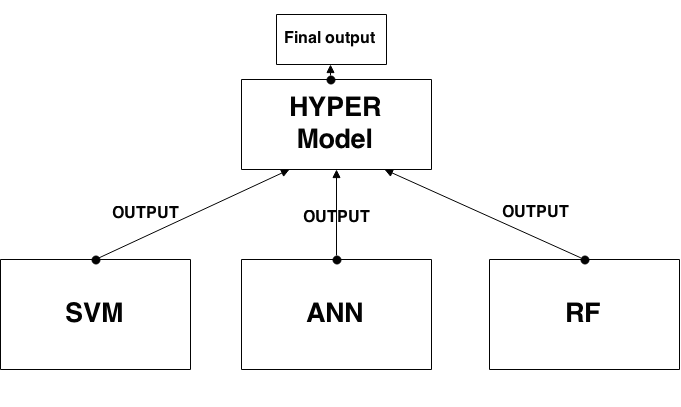
\includegraphics[scale=0.5, keepaspectratio]{Untitled_Diagram.png}
\label{fig:my_label}
\end{figure}


\subsection{Experiment Results}

\subsubsection{Validation Error}

    The Table below is the accuracy rate of model we test on our validation set.
    For support vector machine and  random forest, we conduct n folder validation test, and artificial neural networks we perform batch validation test, which has the same concept of the above method, however it's more efficient when we are doing optimization(mini-batch gradient decent). The reason why we do not use the same method for all models is that different optimization approaches they have have different structures restricting for certain flexibilities. 
    We also present the statistics of our generation process to show whether the generated validation error is a descent proxy for out of sample error.
    

\begin{table}[h]
\centering
\begin{tabular}{|c|l|l|l|}
\hline
\multicolumn{1}{|l|}{Average Validation Errors} & SVM     & ANN    & RF     \\ \hline
Data1                                                  & 23.50\% & 40.0\% & 29.1\% \\ \hline
Data2(PCA, n=20)                                       & 23.75\% & 34.0\% & 27.5\% \\ \hline
Data3(PCA, n=8)                                        & 31.75\% & 2.0\%  & 35.4\% \\ \hline
Data4(PCA, n=20)                                       & 25.5\%  & 40.0\% & 23.6\% \\ \hline
\end{tabular}

\end{table}

    As you can see, the result is frustrating, the errors is some where around 50\% that means our model can not beat the random guess.
    And we next conduct some tests to see what we can improve in next experiment.


\subsubsection{Confusion Mtrices}
What label our model predict wrongly?
\subsection{Feature Selection}
\subsection{Summary for Experiment 1}
1.We should select more meaningful feature to help us to explore the promising features.

2.The frequency of label is too high, and the pattern of label is noisy. We should define the 'answer' more carefully.

3.The feature selection result shows that coil oil price maybe a light of exchange rate prediction.

4. The hourly prediction is merely impossible for economic variables.

5. The result shows that Conditional Restricted Boltzmann machine maybe perform better than the traditional time series process.

\section{Experiment 2}

\subsection{Data description}
We collect the following data from Thomas Routers Data Stream database.
    We divide the factors into different aspects which may affect the exchange rate.


\begin{enumerate}
\item{Stock Market Indice}

\begin{enumerate}
    \item{S&P 500 Index}
    \item{Dow Jons Index}
    \item{Euro stoxx 50 }
    \item{Deutscher Aktienindex}
    \item{France Cotation Assistée en Continu 40}
    \item{NASCOMP}
    \item{Nikki}
\end{enumerate}

\item{Bond Market}
\subitem{}
\subitem{}
\item{Money Supply}
\item{Commodity}

\item{Other Indice}

\end{enumerate}
\newpage
    We describe our data as the market information. 


\subsection{Labeling}

    In Experiment 2 we present two labeling approach. From previous Experiment 1, we know something about that it is very difficult to predict the price movement by economic variables, however it might be result from the factors we select did not contain the crucial information about the price movement, or otherwise from efficient market hypothesis, it is not possible for people gain from historical information under weak form of market efficiency.
    
    Second we construct a equally weighted foreign exchange carry portfolio. From the Experiment 1 we calculate the movement of exchange rate by testing whether the current ask price is higher than the future bid price. The method may result  very noisy labeling pattern, which economic factors cannot catch. To prevent the chaotic pattern we construct a portfolio for our labeling target.
    
    Third we use daily frequency. The lower frequency maybe improve the performance of model.
    
    For label 1 we inherent the method from Experiment 1.The procedure is as follow.
We calculate the daily return of our representative portfolio
if the return is negative we label it as -1 then, positive as +1.

    For label 2, we assume there is impossible for us to predict the daily return movement. So we construct a totally different labeling method. CAPM supports that only systematic risk will be compensated, if CAPM holds the daily return of the market portfolio will explain the daily return. What if we can predict the covariance movement of the portfolio ? Can we beat the market?
    
\subsubsection{Market Correlation Coefficient Matrix}
    We define the market correlation coefficient matrix is the correlation matrix of 7 pairs of currency against GBP. The reason why we use GBP because United Kingdom have higher and more stable interest rate than average country, making interest spread higher. The naive  correlation matrix is calculated as follow.
    $$\rho (x_{i,T},x_{j,T}) = \frac{1}{l}\sum^{T}_{t=T-l}(x_{i,T-t} - \bar{x_{i}})(x_{j,T-t}-\bar{x_{j}})$$
    For our experiment this is totally wrong, and is not a consistent estimator of our market correlation coefficient matrix. What is our target parameter? $\rho(x_{i,t},x_{j,t}) \forall i \not j$ is what we are interested in. The equation above has shown that all we needed is that use past experience to estimate it, however that just show how innocent we are. That means we believe the past experience will happen again, which is not. The newly define market correlation matrix is rewritten as below.
    
    $$\rho (x_{i,T},x_{j,T}) = \frac{1}{l+f}\sum^{T+f}_{t=T-l}(x_{i,T-t} - \bar{x_{i}})(x_{j,T-t}-\bar{x_{j}})$$
    
    This estimator is consistent for market correlation coefficient, however we cannot get at time T, and the idea is somehow connect to local learning. CRBM maybe a promising estimation for the market correlation matrix.
    
\subsubsection{Market Momentum}

We define the market momentum as the distance between the market correlation matrix and the identity matrix. We use euclidean space as our metric space. The different metric space will result different strategy performance. For a baseline we use euclidean space.
    $$d(\rho(x_{t}), \mathbf(I))$$
    There are some economics features about market momentum. It is a proxy for risk in risk out.
    
\begin{figure}
\caption{Market Momentum Histogram}
\centering
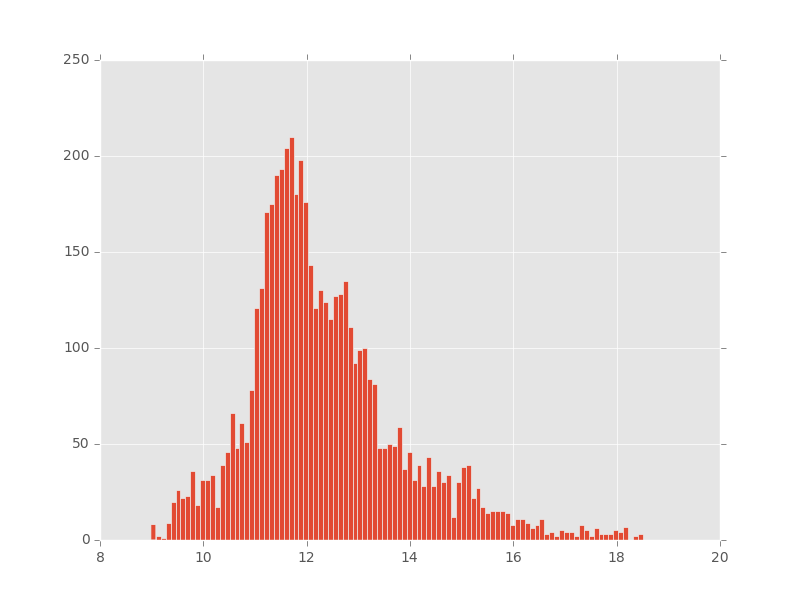
\includegraphics[scale=0.5, keepaspectratio]{market_momentum.png}
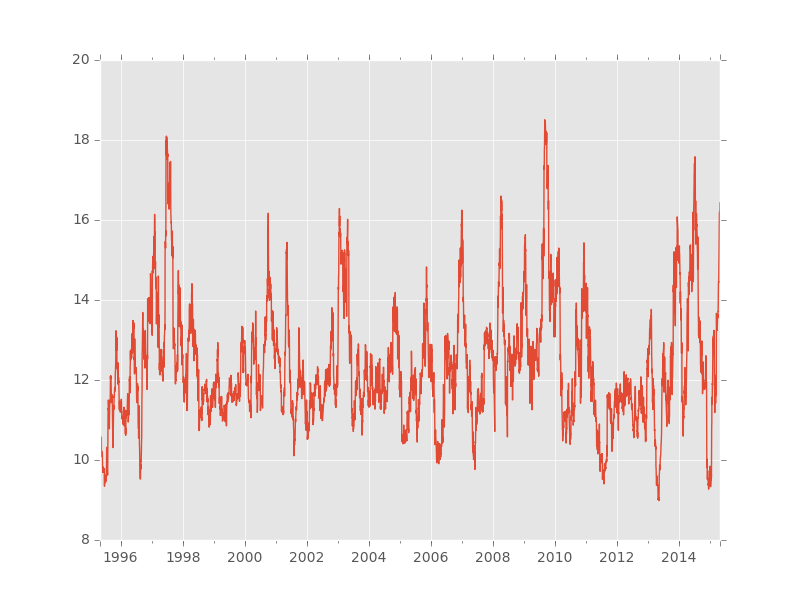
\includegraphics[scale=0.5, keepaspectratio]{historial_market_momentum.png}
\label{fig:my_label}
\end{figure}


\subsubsection{Mixing the whole idea}
    Our Experiment2 present a new designed labeling techniques, the procedure is as follow. We calculate the market momentum, then if the market momentum is greater than it's 25\% quantile  than we label as 1 others we label as 0.
    Is it valid for us to use quantile as a threshold? We found that the time-variant distribution of market momentum is very stable.

\subsection{Data Pre-process}
    Corresponding to the previous experiment, we conduct the same data pre-process methods.  
    
\begin{table}[h]
\centering
\begin{tabular}{|l|l|l|l|l|}
\hline
      & Data              & Process1    & Process2      & Process2 \\ \hline
Data1 & With Lag-terms    & None        & None          & None     \\ \hline
Data2 & With Lag-terms    & PCA         & None          & None     \\ \hline
Data3 & Without Lag-terms & Standardize & 1-layer CRBM(6-Delay)  & PCA      \\ \hline
Data4 & Without Lag-terms & PCA         & None          & None     \\ \hline
\end{tabular}
\end{table}



\subsection{Result}

The training result is shown below.
\subsubsection{Validation Error}

\begin{table}[h]
\centering
\begin{tabular}{|l|l|l|l|l|}
\hline
      & Data              & Process1    & Process2      & Process2 \\ \hline
Data1 & With Lag-terms    & None        & None          & None     \\ \hline
Data2 & With Lag-terms    & PCA         & None          & None     \\ \hline
Data3 & Without Lag-terms & Standardize & 1-layer CRBM(6-Delay)  & PCA      \\ \hline
Data4 & Without Lag-terms & PCA         & None          & None     \\ \hline
\end{tabular}
\end{table}
    The result is very promising. It is possible for us to predict the future market momentum. 

    There are few interesting thing has shown on the result. As we use CRBM as an autoencoder of our data set the error rate is higher than the others data sets. There are few explanation of the difference. 
    First, the historical path of the economics variables has no information of the future market momentum. 
    Second is the CRBM is under fitting, as the data set 1 has reached to $ $ error rate, under the hypothesis that historical path is very important for making prediction on market momentum, it is less likely to have a low accuracy rate of the CRBM than the others discriminative model.

    Since our experiment is extremely successful. This might impose that human portfolio mangers may be defeated by the machine experts which are designed by machine learning experts. The intuition behind the label which predict by the machine can be seen as a risk metric.


\subsection{Test set}


\subsubsection{Currency portfolio}
We choose 7 pairs of currency to form our equally-weighted portfolio.
First benchmark is that we just hold the portfolio for long term.
Second benchmark is the VIX trading strategy, if the VIX index fall below its $0.25$ quantile, we long the equally-weighted portfolio, vise versa.
\subsubsection{Forex carry portfolio}


We also apply the label in our simple strategy. If the model predicts 1 which means that that the market momentum is strengthen by the current market conduction, we would have a long position on risk free rate. If the model predicts 0 then we hold the equally-weighted portfolio. The accumulated sum of the daily return is illustrated in graph. We do not present the further test on our strategy because that is not our focus in this paper.

\subsection{Conclusion}

\subsection{Further Works}
Label serve as a new risk metric{predict daily currency movement}
Test the strategy performance.
Different markets.
Correlation coefficient matrix prediction and estimation.
Optimal portfolio with conditional predictability.
Testing CAPM.
Testing Consumption-based asset pricing model.


